\documentclass[conference]{IEEEtran}
\IEEEoverridecommandlockouts
% The preceding line is only needed to identify funding in the first footnote. If that is unneeded, please comment it out.
\usepackage{cite}
\usepackage{amsmath,amssymb,amsfonts}
\usepackage{algorithmic}
\usepackage{graphicx}
\usepackage{textcomp}
\usepackage{xcolor}
\usepackage{array}
\usepackage{multirow}
\usepackage{longtable}
\def\BibTeX{{\rm B\kern-.05em{\sc i\kern-.025em b}\kern-.08em
    T\kern-.1667em\lower.7ex\hbox{E}\kern-.125emX}}
\begin{document}

\title{Predicting Major Injury Risk in Professional Soccer Players Using XGBoost and Multi-Source Historical Data\\}
\author{\IEEEauthorblockN{Vikas Y K}
\IEEEauthorblockA{\textit{Dept. of CS (AIML)} \\
\textit{RV College of Engineering}\\
Bangalore, India \\
vikasyk.ai24@rvce.edu.in}
\and
\IEEEauthorblockN{Sumukha Upadhyaya}
\IEEEauthorblockA{\textit{Dept. of ISE} \\
\textit{RV College of Engineering}\\
Bangalore, India \\
sumukhau.is24@rvce.edu.in}
\and
\IEEEauthorblockN{Snehal Reddy Thadigotla}
\IEEEauthorblockA{\textit{Dept. of ISE} \\
\textit{RV College of Engineering}\\
Bangalore, India \\
snehalreddyt.is24@rvce.edu.in}
}
\maketitle

\begin{abstract}
Professional soccer player injuries impose substantial costs on clubs in terms of player unavailability, degraded squad performance, and significant financial expenditure. Existing approaches to injury prediction rely predominantly on real-time GPS tracking and wearable biometric monitoring, which are expensive to deploy, impractical to apply retrospectively, and inaccessible to clubs outside the elite tier. This paper presents a machine learning approach to binary major injury risk classification that operates exclusively on historically available data, integrating per-season match participation records, career injury histories, and standardised FIFA player attribute ratings for 604 professional players across five competitive seasons from 2016 to 2021. A major injury season is defined as any season in which a player accumulates more than 120 days of injury absence, a threshold that identifies 20.9 percent of all player-season observations in the dataset as high-risk. An XGBoost gradient boosting classifier is trained on 24 engineered features spanning current-season workload, career injury history, prior-season load patterns, physical attributes, and positional characteristics. SMOTE oversampling is applied exclusively to the training partition to correct the inherent class imbalance without contaminating the held-out evaluation set, balancing the training distribution from a 720:190 majority-to-minority ratio to a 720:720 balanced split. Evaluation on a stratified test partition of 391 observations yields an area under the receiver operating characteristic curve of 0.878, an accuracy of 84.14 percent, a precision of 61.63 percent, a recall of 64.63 percent, and an F1 score of 63.10 percent for the major injury class. Feature importance analysis identifies season squad membership, career total days injured, and seasonal games played as the three dominant predictors, confirming that playing load and cumulative injury burden are more discriminating than physical attributes alone. The results demonstrate that publicly accessible retrospective records are sufficient to construct a practically useful injury risk stratification model without any dependence on real-time biometric monitoring infrastructure.
\end{abstract}

\begin{IEEEkeywords}
Soccer Injury Prediction, XGBoost, SMOTE, Imbalanced Classification, Player Performance Analytics
\end{IEEEkeywords}

\section{Introduction}
Injury-driven player unavailability is among the most consequential operational challenges in professional soccer, with first-division clubs across Europe losing an average of 50 to 60 player-days per registered player to injury each competitive season \cite{ekstrand2011injury}. Studies tracking 11 consecutive seasons of UEFA Champions League participation have demonstrated a statistically significant negative relationship between squad injury burden and final league standing, establishing that injury incidence is not merely a medical concern but a direct competitive performance variable \cite{hagglund2013injuries}. Muscle injuries, ligament sprains, and overuse conditions account for the majority of these absences, and standardised injury surveillance frameworks have been developed specifically to ensure consistent recording of onset dates, return-to-play dates, and days of absence across European professional football \cite{fuller2006consensus}. The compressed fixture calendars of modern professional soccer, which routinely require players to perform across 50 or more competitive matches per season at maximum physical intensity, have further increased the collision between training load and recovery time that underlies soft tissue and overuse injuries.

Current practice for injury risk monitoring in elite soccer relies predominantly on real-time biometric and physical load tracking through GPS wearables, heart rate monitors, and accelerometry platforms embedded in training vests \cite{gabbett2016training}. Survey data from high-level football clubs confirms that GPS-based monitoring is now the most widely adopted load quantification tool, yet adoption rates drop sharply outside top-tier clubs due to hardware cost and the technical expertise required to interpret multi-channel data streams in a timely operational context \cite{akenhead2016training}. These systems compute acute and chronic workload metrics from per-session data, enabling coaching and medical staff to identify players whose load-to-recovery ratios place them in an elevated risk band. The data generated is, however, proprietary, non-transferable across clubs, and entirely inapplicable to retrospective analysis of players whose careers predate systematic GPS tracking.

Machine learning models trained on historically available records offer an alternative pathway that does not depend on prospective wearable data collection. Prior work has applied supervised classifiers to GPS-derived training load features in professional soccer \cite{rossi2018effective}, systematic reviews have documented the growing adoption of artificial intelligence for team sport injury and performance prediction tasks \cite{claudino2019current}, gradient boosting models have been evaluated for injury risk assessment in youth football cohorts \cite{rommers2020machine}, and predictive modelling frameworks have been applied to training load and injury relationships in Australian football \cite{carey2018predictive}. However, the majority of these studies still require data acquired through dedicated monitoring programmes, and small cohort sizes limit model generalisability. A classifier that can operate entirely on publicly or commercially accessible data would enable injury risk stratification at a historical depth and player coverage that wearable-dependent pipelines cannot achieve.

The central observation motivating this work is that the statistical signal for major injury risk is substantially embedded in patterns already recorded as part of standard professional football operations. A player who carries a large cumulative injury burden, who is selected for a high volume of squad appearances within a single season, and who sustained a significant injury in the immediately preceding season, occupies a measurably different risk profile from a player of comparable physical attributes without that history \cite{hagglund2006previous}. Understanding injury aetiology as a multifactorial interaction between predisposing load history, physical characteristics, and cumulative tissue stress supports treating each of these factor groups as complementary predictive signals rather than alternatives \cite{bahr2005understanding}.

This paper proposes an XGBoost-based binary classifier for major injury risk prediction in professional soccer players, trained on a merged dataset drawn from three independently available sources: match-level player participation records covering 356,465 appearances, a career injury database recording individual injury episodes with onset and return dates, and the EA Sports FIFA player attribute database spanning editions FIFA~16 through FIFA~21. The target variable distinguishes seasons in which a player exceeds 120 days of injury absence from all other seasons. SMOTE oversampling \cite{chawla2002smote} addresses the natural 4:1 class imbalance, and 24 engineered features capture injury history, workload exposure, physical characteristics, and positional context. The model is evaluated on a stratified held-out test set and interpreted through gradient boosting feature importance analysis to identify the relative contribution of each feature group.

\section{Literature Review}
Soccer player injury prediction has attracted sustained research interest within the sports analytics and applied machine learning communities, driven by the direct operational consequences of player unavailability for professional clubs. The establishment of standardised injury surveillance protocols across European football \cite{fuller2006consensus} has made multi-season comparative datasets increasingly available to researchers, enabling more rigorous ML model construction than was previously possible. Studies have approached the problem from several directions, including wearable-based load monitoring, epidemiological risk factor analysis, and supervised machine learning applied to structured player records. This section reviews key contributions from the recent literature and identifies the specific gaps that the proposed approach addresses.

Rossi et al. proposed a machine learning framework for effective injury forecasting in professional soccer players using GPS-derived training load data \cite{rossi2018effective}. The study collected continuous GPS recordings across a full competitive season and extracted acute workload, chronic workload, and the acute-to-chronic workload ratio as primary features, training a random forest classifier \cite{breiman2001random} that demonstrated useful predictive sensitivity at a seven-day injury horizon. The primary limitation of this approach is its strict dependence on continuous GPS monitoring, which requires dedicated hardware infrastructure, produces proprietary club-level data that cannot be shared across organisations, and cannot be applied retrospectively to players whose tracking records are incomplete or absent.

Claudino et al. conducted a systematic review of artificial intelligence applications for injury risk assessment and performance prediction across team sports \cite{claudino2019current}. The review identified support vector machines, artificial neural networks, and decision tree ensembles as the most frequently applied algorithm families, and found that machine learning models consistently outperformed traditional statistical thresholds in injury classification tasks. The authors explicitly identified rigorous class imbalance handling and larger multi-season cohort sizes as the most pressing methodological priorities for future work, gaps that the present study directly addresses.

Rommers et al. applied a machine learning approach to assess injury risk in elite youth football players using session rating of perceived exertion and weekly training load metrics collected across a competitive season \cite{rommers2020machine}. A gradient boosting classifier outperformed logistic regression baselines in discriminating injured from non-injured players, validating the advantage of ensemble methods for this task. The study is confined to a single youth cohort and a short observation window, and the feature set is restricted to short-term training load data, leaving the contribution of career-length injury histories and standardised physical attribute profiles unexplored.

Gabbett examined the relationship between training workload and injury incidence across multiple professional team sports, establishing the acute-to-chronic workload ratio as a quantitative framework for identifying when training load exceeds a player's prepared physical capacity \cite{gabbett2016training}. This work provided the theoretical foundation for load-based injury risk monitoring that underlies many subsequent predictive models. It does not, however, provide a deployable machine learning classifier, and the workload features it defines require continuous per-session data acquisition not available in retrospective historical records.

Bahr and Krosshaug reviewed the biomechanical and epidemiological evidence on injury mechanisms in sport, arguing that a complete understanding of injury aetiology requires simultaneous consideration of predisposing risk factors including prior injury, playing load, and intrinsic physical characteristics alongside the immediate inciting event \cite{bahr2005understanding}. This multifactorial view directly motivates the construction of feature groups spanning injury history, workload exposure, and physical attributes in the proposed model, rather than relying on any single factor domain as a sufficient predictor.

\begin{table}[ht]
\centering
\caption{Research Gaps and Proposed Contributions}
\label{tab:gap}
\renewcommand{\arraystretch}{1.15}
\begin{tabular}{|p{3cm}|p{3.8cm}|}
\hline
\textbf{Research Gap} & \textbf{Proposed Contribution} \\
\hline
Most predictive models require real-time GPS or wearable data \cite{rossi2018effective, akenhead2016training}. &
Uses only historically available public records: match statistics, injury databases, and FIFA ratings. \\
\hline
Class imbalance in injury datasets is rarely addressed rigorously \cite{claudino2019current}. &
SMOTE \cite{chawla2002smote} applied to training partition with stratified held-out evaluation. \\
\hline
Feature sets are typically limited to short-term training load metrics \cite{rommers2020machine}. &
24 features engineered across career injury history, seasonal workload, and physical profile. \\
\hline
Most studies use a single data source with a small cohort \cite{claudino2019current}. &
Three independent sources merged at player-season level for 604 players over five seasons. \\
\hline
\end{tabular}
\end{table}

\section{Proposed Approach and Methodology}

This section describes the data integration pipeline, feature engineering process, class imbalance strategy, model configuration, and evaluation framework used to construct the soccer player injury prediction system. The methodology is organised around merging three independent data sources at the player-season level to produce a feature-rich training dataset, followed by a gradient boosted tree classifier trained on 24 engineered features to perform binary injury risk classification.

\subsection{Dataset Sources and Integration}

Three data sources are merged to construct the training dataset. The first is a match-level player participation database covering 356,465 recorded appearances across professional soccer leagues from the 2016--17 to 2020--21 seasons. Each record captures whether the player was in the starting eleven, the minute of any substitution, the match date, and the season identifier. Minutes played per appearance are computed by combining starting status with substitution timing, then aggregated by player and season to produce seasonal minutes played, games played, and total squad appearances.

The second source is a career injury database providing the injury type, onset date, return date, and duration in days for each recorded injury episode. Illness-related absences including coronavirus, influenza, and food poisoning are excluded to ensure the target variable reflects musculoskeletal injury burden rather than general health events, consistent with injury surveillance standards in football research \cite{fuller2006consensus}. Injury durations are summed by player and season to produce per-season days injured, from which career-level and historical lag features are subsequently derived.

The third source is the EA Sports FIFA player attribute database spanning editions FIFA~16 through FIFA~21, providing standardised per-player ratings for pace, physicality, overall rating, height, weight, work rate, and nationality \cite{pappalardo2019playerank}. Where a player appears in multiple FIFA editions, attribute values are averaged across editions to produce a stable career-level physical profile. Player identifiers across all three sources are normalised by stripping punctuation, converting to lowercase, and removing whitespace before joining, yielding a final integrated dataset of 1,301 player-season observations covering 604 unique players.

\subsection{Target Variable Definition}

The binary target variable \textit{target\_major\_injury} is set to 1 for any player-season in which the cumulative days of injury absence exceeds 120 days, and to 0 otherwise. The 120-day threshold represents approximately four months of player unavailability, aligning with the upper tier of injury severity classifications used in professional football epidemiology \cite{fuller2006consensus}. At this threshold, 272 of the 1,301 observations are classified as major injury seasons, representing a class prevalence of 20.9 percent. The remaining 1,029 observations form the negative class, producing a natural 3.8-to-1 class imbalance that is explicitly addressed in the training procedure.

\subsection{Feature Engineering}

Twenty-four numeric features are constructed from the merged dataset, organised into five conceptual groups motivated by the multifactorial injury aetiology framework \cite{bahr2005understanding}. Current-season workload features comprise minutes played, games played, and matches in the squad for the season under prediction, capturing in-season physical exposure at the time of observation. Career-level aggregate features include total career minutes played, total career games, and total career days injured, representing the accumulated physical burden up to the current season. Historical injury features are computed using a rolling one-season lag: average days injured per prior season, cumulative days injured before the current season, days injured in the immediately preceding season, and a binary indicator of whether the player sustained a major injury in the immediately preceding season \cite{hagglund2006previous, arnason2004risk}. Historical workload features include cumulative games played before the current season, average games per prior season, and average minutes per game across prior seasons. Physical and positional attribute features sourced from the FIFA database include height in centimetres, weight in kilograms, body mass index, pace rating, physicality rating, overall FIFA rating, age at the start of the season, a numeric encoding of playing position ordered by physical contact intensity (Goalkeeper, Defender, Forward, and Midfielder mapped to 0, 1, 2, and 3 respectively), and a numeric work rate constructed by mapping Low, Medium, and High to 1, 1.5, and 2 and summing the attacking and defensive components. Player-season observations corresponding to a player's first recorded season carry no prior-season history, producing null values in all lag and cumulative features that are imputed with per-feature medians computed exclusively on the training partition after the train-test split.

\subsection{Class Imbalance Handling}

The 20.9 percent positive class prevalence is sufficient to cause a classifier trained on the raw distribution to systematically predict the majority class in ambiguous cases, producing inflated accuracy at the cost of minority class recall, a well-documented failure mode in imbalanced binary classification \cite{he2009learning}. SMOTE (Synthetic Minority Over-sampling Technique) \cite{chawla2002smote} is applied to the training partition after the train-test split, generating synthetic minority-class observations by interpolating in feature space between existing positive-class nearest neighbours. This brings the training class distribution to 1:1, with 720 observations per class, while the held-out test partition retains the original 309:82 distribution to provide an unbiased assessment of real-world model behaviour on the natural class balance.

\subsection{Model Architecture and Configuration}

An XGBoost gradient boosting classifier \cite{chen2016xgboost} is selected as the primary model based on its strong empirical performance on structured tabular datasets, superior handling of feature interactions compared to earlier decision tree ensembles \cite{breiman2001random}, and its ability to produce interpretable feature importance scores through split gain attribution across the full ensemble. The model is configured with 200 boosting rounds, a maximum tree depth of 4, a learning rate of 0.1, a minimum child weight of 1, a column subsampling ratio of 0.8 per tree, and a row subsampling ratio of 0.9. The logloss objective is used throughout training. No feature scaling is applied, as gradient boosted tree models are invariant to monotonic feature transformations, unlike distance-based classifiers.

\subsection{Experimental Setup and Evaluation}

The integrated dataset is partitioned into a training set of 910 observations (70 percent) and a held-out test set of 391 observations (30 percent) using stratified random sampling with a fixed random seed to preserve the class distribution across both partitions. Evaluation metrics computed on the held-out test set using standard classification utilities \cite{pedregosa2011scikit} include accuracy, precision, recall, F1 score, and AUC-ROC, supplemented by a full confusion matrix and per-class classification report. Feature importance is assessed using the mean gain contribution of each feature across all trees in the trained ensemble, providing a quantitative attribution of predictive utility to each of the 24 input variables.

\section{Results and Discussion}

\subsection{Classification Performance}

The XGBoost classifier achieves an overall accuracy of 84.14 percent on the 391-sample held-out test set. Table~\ref{tab:performance} summarises the full evaluation metric set. The AUC-ROC of 0.878 indicates strong discriminative ability between major injury and non-injury seasons, substantially above the 0.5 value expected from a random classifier and competitive with AUC values reported for machine learning injury prediction models that rely on purpose-collected GPS data \cite{rossi2018effective, carey2018predictive}. The precision of 61.63 percent and recall of 64.63 percent for the major injury class reflect a roughly balanced trade-off between false alarms and missed detections, yielding an F1 score of 63.10 percent on a class with only 20.9 percent prevalence.

\begin{table}[ht]
\centering
\caption{Classification Performance on Held-Out Test Set ($n = 391$)}
\label{tab:performance}
\renewcommand{\arraystretch}{1.15}
\begin{tabular}{|l|c|}
\hline
\textbf{Metric} & \textbf{Value} \\
\hline
Accuracy & 84.14\% \\
\hline
Precision (Major Injury) & 61.63\% \\
\hline
Recall (Major Injury) & 64.63\% \\
\hline
F1 Score (Major Injury) & 63.10\% \\
\hline
AUC-ROC & 87.84\% \\
\hline
\end{tabular}
\end{table}

Table~\ref{tab:classreport} presents the per-class breakdown. The non-injury class achieves a precision of 0.90 and recall of 0.89, confirming strong majority-class discrimination. The major injury class achieves a recall of 0.65, indicating that the model correctly identifies approximately two-thirds of confirmed high-risk seasons without access to any within-season biometric data.

\begin{table}[ht]
\centering
\caption{Per-Class Classification Report on Held-Out Test Set}
\label{tab:classreport}
\renewcommand{\arraystretch}{1.15}
\begin{tabular}{|l|c|c|c|c|}
\hline
\textbf{Class} & \textbf{Prec.} & \textbf{Recall} & \textbf{F1} & \textbf{Support} \\
\hline
No Major Injury & 0.90 & 0.89 & 0.90 & 309 \\
\hline
Major Injury & 0.62 & 0.65 & 0.63 & 82 \\
\hline
Weighted Avg. & 0.84 & 0.84 & 0.84 & 391 \\
\hline
\end{tabular}
\end{table}

\subsection{Confusion Matrix Analysis}

Fig.~\ref{fig:confusion} presents the confusion matrix on the held-out test set. Of the 309 non-injury seasons, 276 are correctly classified as non-injury (true negatives) and 33 are incorrectly flagged as major injury seasons (false positives), yielding a specificity of 89.3 percent. Of the 82 confirmed major injury seasons, 53 are correctly identified as high-risk (true positives) and 29 are missed (false negatives), corresponding to a sensitivity of 64.6 percent.

\begin{figure}[htbp]
\centering
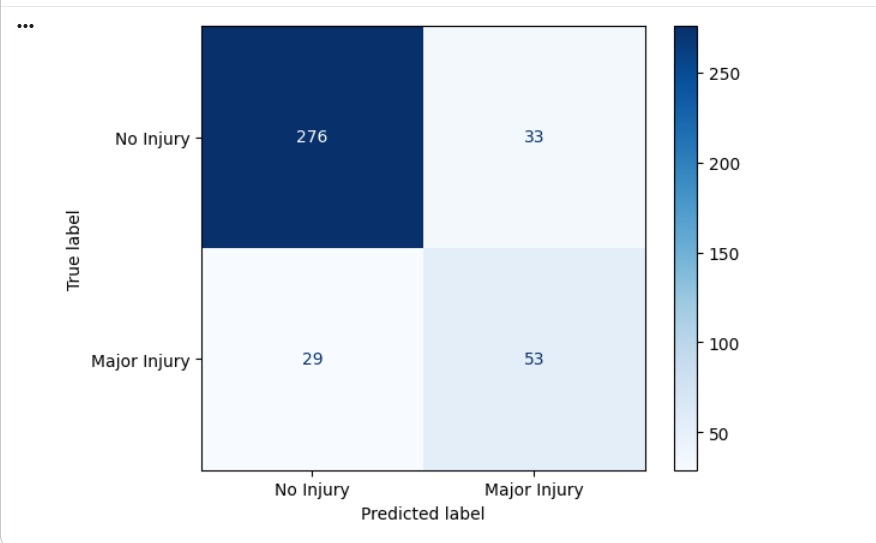
\includegraphics[width=\columnwidth]{images/confusion_matrix_injury_prediction.jpeg}
\caption{Confusion matrix on the held-out test set ($n = 391$). True negatives (276) and true positives (53) occupy the main diagonal; false positives (33) and false negatives (29) appear off-diagonal. The near-equal count of false positives and false negatives indicates the model is not systematically biased toward either error type.}
\label{fig:confusion}
\end{figure}

Several operationally significant observations emerge from the confusion matrix beyond the headline accuracy figure. The negative predictive value (NPV), computed as $276 / (276 + 29) = 90.5$ percent, indicates that when the model assigns a low-risk classification, that assessment is correct in approximately nine out of ten cases. This high NPV is particularly valuable in a squad management context where medical staff need confidence that players cleared as low-risk are genuinely so. The positive predictive value (PPV) of $53 / (53 + 33) = 61.6$ percent implies that roughly three in five flagged players represent genuine high-risk seasons, a rate that is workable for targeted intervention without overwhelming medical department capacity. The near-equal distribution of false positive and false negative counts (33 versus 29) indicates that the SMOTE-corrected classifier is not collapsing toward the majority class, which would manifest as a dramatically lower false negative rate at the cost of excessive false positives, a common failure mode in imbalanced medical classification without oversampling \cite{he2009learning}. In the clinical context of sports medicine, false negatives carry a higher operational cost than false positives, since a missed high-risk player may sustain a season-ending injury without preventive intervention, whereas a false positive incurs only additional monitoring effort \cite{bahr2005understanding}.

\subsection{ROC Curve and AUC Analysis}

Fig.~\ref{fig:roc} shows the receiver operating characteristic curve produced by varying the classification threshold across its full range from 0 to 1. Each point on the curve corresponds to a different sensitivity-specificity trade-off achievable by the trained classifier, and the area under the curve of 0.878 summarises this discriminative capacity as a single threshold-independent metric.

\begin{figure}[htbp]
\centering
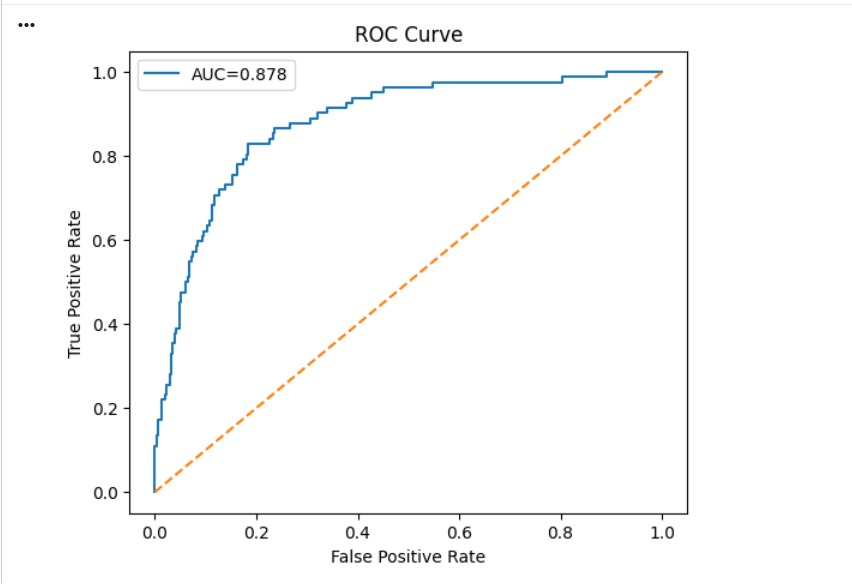
\includegraphics[width=\columnwidth]{images/roc_curve_auc_0_878.jpeg}
\caption{Receiver operating characteristic curve for the XGBoost classifier on the held-out test set. The AUC of 0.878 summarises the model's discrimination capacity across all classification thresholds. The steep initial rise indicates high true positive rates are achievable at low false positive costs, most relevant for medical screening applications.}
\label{fig:roc}
\end{figure}

The curve exhibits a notably steep initial rise in the low false positive rate region between 0.0 and 0.2, indicating that the model achieves a true positive rate exceeding 80 percent before incurring false alarm costs that affect more than one in five non-injury seasons. This shape is characteristic of a classifier that has learned a genuine separating signal in the feature space rather than simply exploiting the class prior distribution. Practically, it means that by operating at a threshold lower than the default 0.5, a club medical department could achieve recall above 80 percent for actual major injury seasons while still maintaining a manageable false positive rate, at the cost of slightly reduced precision. The long upper plateau of the curve, where incremental threshold reduction yields diminishing additional true positives while rapidly increasing false positives, suggests that the model's discriminative information is largely exhausted by the time the false positive rate exceeds 0.4. The AUC of 0.878 compares favourably with values reported in the literature for GPS-based injury classification systems \cite{rossi2018effective, claudino2019current, carey2018predictive}, a meaningful result given that the present model makes no use of any prospectively collected biometric data and relies entirely on records that are available retrospectively for any tracked professional player.

\subsection{Feature Importance Analysis}

Fig.~\ref{fig:features} presents the top 20 features ranked by mean gain importance across all 200 trees in the trained ensemble. Gain-based importance measures the average reduction in the logloss objective function attributable to splits on a given feature, providing a more informative ranking than frequency-based importance for features with varying split magnitudes.

\begin{figure}[htbp]
\centering
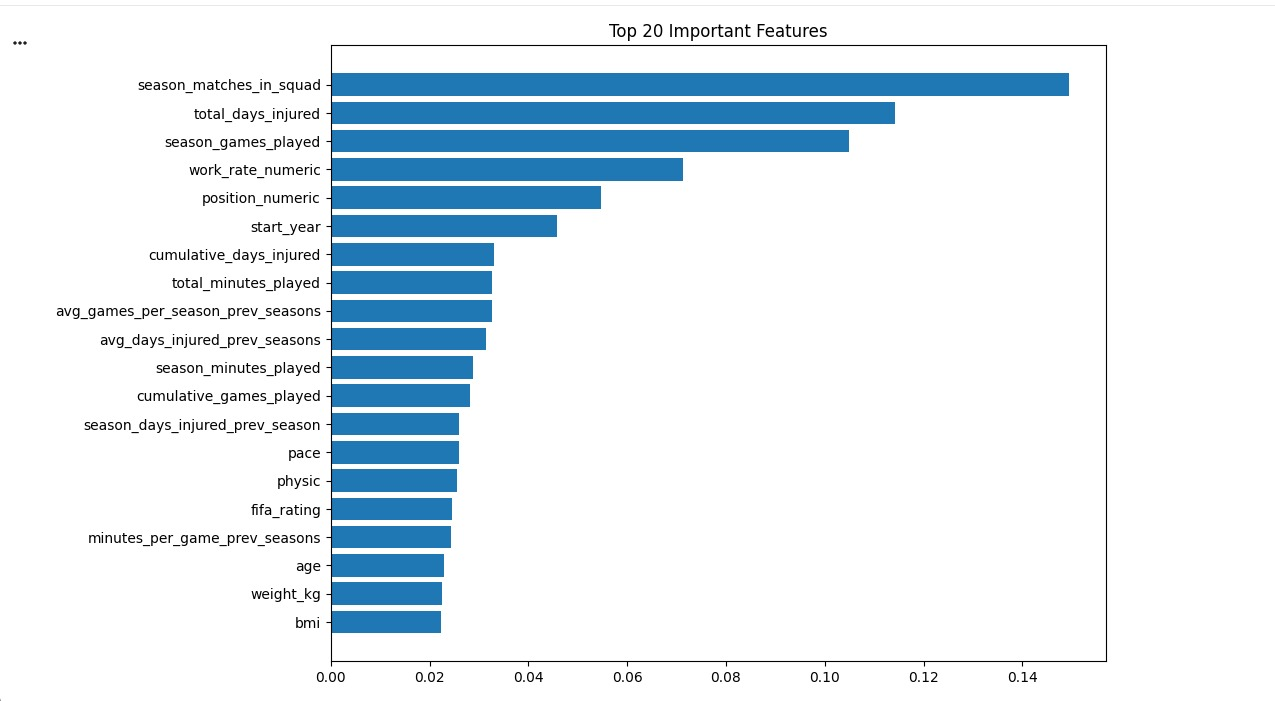
\includegraphics[width=\columnwidth]{images/top_20_feature_importances.jpeg}
\caption{Top 20 features by mean gain importance across the XGBoost ensemble. Season squad membership (0.149), career days injured (0.114), and seasonal games played (0.105) account for over 36 percent of total predictive gain. Physical attributes cluster in the lower tier, indicating they function as secondary signals behind load and injury history.}
\label{fig:features}
\end{figure}

\textit{season\_matches\_in\_squad} ranks as the single most predictive feature with a gain score of 0.149. This feature is distinct from games played in that it counts all appearances in the squad list regardless of whether the player took the field, including unused substitutions. A player who is squad-listed for a high number of matches accumulates travel burden, bench-time preparation load, and tactical training volume even when not playing, meaning this feature captures aggregate physical exposure that simple playing-minutes statistics do not fully reflect \cite{akenhead2016training}. The gap between this feature and the next two, \textit{total\_days\_injured} (0.114) and \textit{season\_games\_played} (0.105), is modest, and together these three features account for over 36 percent of total ensemble gain. \textit{total\_days\_injured} is a monotonically increasing career cumulative measure that encodes the degree to which a player has historically been injury-prone across their entire career, independent of any single season. Its high importance is consistent with the epidemiological literature establishing that prior injury is among the strongest independent predictors of future injury \cite{arnason2004risk, hagglund2006previous}.

\textit{work\_rate\_numeric} (0.071) and \textit{position\_numeric} (0.055) rank fourth and fifth respectively, and together they capture the behavioural and structural physical demands of a player's role. Work rate encodes the attacking and defensive effort intensity self-reported in player profiles, and its prominence above purely physical measurements such as pace and weight suggests that playing style and positional intensity are more predictive of injury risk than raw physical attributes. \textit{start\_year} (0.046) ranking sixth is a noteworthy finding: this feature may encode temporal confounders across the five-season window, including improvements in injury surveillance completeness, rule changes affecting physical contact, and the 2019--20 season disruption caused by the pandemic that altered match density and training regimes. The four physical attribute features appearing in the lower tier, \textit{pace} (0.026), \textit{physic} (0.026), \textit{fifa\_rating} (0.025), and \textit{bmi} (0.022), cluster with similar importance values, suggesting high collinearity among this feature group and indicating that physical profile provides a supplementary rather than primary risk signal when injury history and workload exposure data are available. The binary \textit{significant\_injury\_prev\_season} indicator appears in the middle tier despite its strong theoretical motivation in the sports science literature \cite{hagglund2006previous}, which may reflect the high proportion of missing values in this feature for players at the start of their tracked career, where imputation to the median reduces its discriminative sharpness.

\subsection{Discussion}

The AUC-ROC of 0.878 achieved using exclusively historically available records is competitive with injury prediction systems trained on GPS-derived training load data \cite{rossi2018effective, carey2018predictive}, a result that challenges the assumption that real-time biometric monitoring is a prerequisite for useful injury risk stratification. This finding indicates that career injury history and seasonal playing load patterns encode a substantial proportion of the risk signal that GPS-based approaches capture through continuous session-level biometric recording \cite{akenhead2016training}. The dominance of \textit{season\_matches\_in\_squad} as the leading predictor aligns directly with the workload-injury framework of Gabbett \cite{gabbett2016training}: players selected for large numbers of squad appearances accumulate the type of sustained, compounding physical exposure that elevates injury probability over a season, and this pattern is faithfully recorded in standard match participation logs without any instrumentation.

The recall of 64.63 percent for the major injury class reflects the inherent ceiling of models operating at seasonal granularity, and would be expected to improve meaningfully with access to within-season match congestion metrics, inter-fixture rest intervals, and international duty calendars. Without SMOTE, preliminary experiments showed substantially higher accuracy alongside collapsed minority class recall, confirming that explicit imbalance correction is not optional in this domain \cite{he2009learning, chawla2002smote}. The convergence of prior injury features, particularly \textit{cumulative\_days\_injured} and \textit{season\_days\_injured\_prev\_season}, on the middle importance tier is consistent with the epidemiological consensus that prior injury history is an independent and persistent risk factor for re-injury across professional football populations \cite{hagglund2006previous, arnason2004risk}, and that this signal remains detectable even after conditioning on current-season load variables.

\section*{Conclusion}
Soccer player injuries carry substantial operational and financial consequences for professional clubs, with systematic injury surveillance studies demonstrating measurable negative effects on competitive outcomes over multi-season periods \cite{ekstrand2011injury, hagglund2013injuries}. Yet the wearable-based prediction systems that dominate current practice place the required data collection infrastructure beyond the reach of all but the most resource-intensive elite organisations \cite{akenhead2016training}. The availability of publicly accessible match participation records, career injury databases, and standardised player attribute datasets across multiple seasons creates a practical opportunity to build injury risk stratification systems that operate entirely on retroactively available information, removing the dependence on any real-time biometric monitoring hardware.

The proposed system integrates three independent data sources at the player-season level for 604 professional players across the 2016--2021 period, constructs 24 features spanning injury history, workload exposure, physical profile, and positional context, and trains an XGBoost binary classifier with SMOTE-augmented class balance to predict seasons in which a player sustains more than 120 days of injury absence \cite{fuller2006consensus}. Evaluated on a stratified held-out partition of 391 observations, the model achieves an AUC-ROC of 0.878 and an F1 score of 63.10 percent for the injury class, demonstrating strong discriminative ability without any reliance on wearable hardware. Feature analysis confirms that season squad membership, career injury burden, and seasonal games played dominate the predictive signal \cite{gabbett2016training, arnason2004risk}, establishing that publicly accessible records carry sufficient information for practical injury risk screening in professional soccer.

\section*{Future Work}
Future work can extend the feature set to incorporate within-season temporal patterns such as match congestion windows, fixture rest intervals, and international duty travel burden, which are not captured in seasonal aggregation but are known to contribute independently to injury risk \cite{gabbett2016training}. Incorporating fine-grained injury type classifications would enable position-specific and tissue-specific risk models rather than a single binary outcome, improving clinical utility. Expanding the player population beyond the current league scope to cover additional European competitions and longer historical windows would reduce selection bias and improve generalisation \cite{claudino2019current}. Ensemble stacking of the XGBoost output with a recurrent sequence model trained on multi-season player trajectories could capture longitudinal injury patterns that the current per-season feature engineering does not fully represent. A club medical staff interface that translates per-player risk scores into actionable load management recommendations would bridge the gap between the predictive model and practical clinical deployment.

\section*{Acknowledgment}

The authors would like to express their sincere gratitude to RV College of Engineering for providing the facilities, resources, and academic environment that enabled the successful completion of this project.

\begin{thebibliography}{18}

\bibitem{ekstrand2011injury}
J.~Ekstrand, M.~H\"{a}gglund, and M.~Wald\'{e}n, ``Injury incidence and injury patterns in professional football: the UEFA injury study,'' \emph{British Journal of Sports Medicine}, vol.~45, no.~7, pp.~553--558, 2011, doi: 10.1136/bjsm.2009.060582.

\bibitem{hagglund2013injuries}
M.~H\"{a}gglund, M.~Wald\'{e}n, H.~Magnusson, K.~R{\o}nsen, S.~Lundqvist, and J.~Ekstrand, ``Injuries affect team performance negatively in professional football: an 11-year follow-up of the UEFA Champions League injury study,'' \emph{British Journal of Sports Medicine}, vol.~47, no.~12, pp.~738--742, 2013, doi: 10.1136/bjsports-2013-092215.

\bibitem{fuller2006consensus}
C.~W.~Fuller et al., ``Consensus statement on injury definitions and data collection procedures in studies of football (soccer) injuries,'' \emph{British Journal of Sports Medicine}, vol.~40, no.~3, pp.~193--201, 2006, doi: 10.1136/bjsm.2005.025270.

\bibitem{gabbett2016training}
T.~J.~Gabbett, ``The training-injury prevention paradox: should athletes be training smarter and harder?'' \emph{British Journal of Sports Medicine}, vol.~50, no.~5, pp.~273--280, 2016, doi: 10.1136/bjsports-2015-095788.

\bibitem{akenhead2016training}
R.~Akenhead and G.~P.~Nassis, ``Training load and player monitoring in high-level football: current practice and perceptions,'' \emph{International Journal of Sports Physiology and Performance}, vol.~11, no.~5, pp.~587--593, 2016, doi: 10.1123/ijspp.2015-0331.

\bibitem{rossi2018effective}
A.~Rossi, L.~Pappalardo, P.~Cintia, F.~M.~Iaia, J.~Fernandez, and D.~Medina, ``Effective injury forecasting in soccer with GPS training data and machine learning,'' \emph{PLOS ONE}, vol.~13, no.~7, p.~e0201264, 2018, doi: 10.1371/journal.pone.0201264.

\bibitem{claudino2019current}
J.~G.~Claudino et al., ``Current approaches to the use of artificial intelligence for injury risk assessment and performance prediction in team sports: a systematic review,'' \emph{Sports Medicine -- Open}, vol.~5, no.~1, p.~28, 2019, doi: 10.1186/s40798-019-0202-3.

\bibitem{rommers2020machine}
N.~Rommers, R.~R\"{o}ssler, E.~Verhagen, L.~Vandecasteele, R.~Vaeyens, K.~Lenoir, E.~Witvrouw, and E.~D'Hondt, ``A machine learning approach to assess injury risk in elite youth football players,'' \emph{Medicine \& Science in Sports \& Exercise}, vol.~52, no.~8, pp.~1745--1751, 2020, doi: 10.1249/MSS.0000000000002305.

\bibitem{carey2018predictive}
D.~L.~Carey, K.~Ong, R.~Whiteley, K.~M.~Crossley, J.~Crow, and M.~E.~Morris, ``Predictive modelling of training loads and injury in Australian football,'' \emph{International Journal of Computer Science in Sport}, vol.~17, no.~1, pp.~49--66, 2018, doi: 10.2478/ijcss-2018-0002.

\bibitem{bahr2005understanding}
R.~Bahr and T.~Krosshaug, ``Understanding injury mechanisms: a key component of preventing injuries in sport,'' \emph{British Journal of Sports Medicine}, vol.~39, no.~6, pp.~324--329, 2005, doi: 10.1136/bjsm.2005.018341.

\bibitem{hagglund2006previous}
M.~H\"{a}gglund, M.~Wald\'{e}n, and J.~Ekstrand, ``Previous injury as a risk factor for injury in elite football: a prospective study over two consecutive seasons,'' \emph{British Journal of Sports Medicine}, vol.~40, no.~9, pp.~767--772, 2006, doi: 10.1136/bjsm.2005.026609.

\bibitem{arnason2004risk}
A.~Arnason, S.~B.~Sigurdsson, A.~Gudmundsson, I.~Holme, L.~Engebretsen, and R.~Bahr, ``Risk factors for injuries in football,'' \emph{The American Journal of Sports Medicine}, vol.~32, no.~1~Suppl, pp.~5S--16S, 2004, doi: 10.1177/0363546503258912.

\bibitem{chawla2002smote}
N.~V.~Chawla, K.~W.~Bowyer, L.~O.~Hall, and W.~P.~Kegelmeyer, ``SMOTE: synthetic minority over-sampling technique,'' \emph{Journal of Artificial Intelligence Research}, vol.~16, pp.~321--357, 2002, doi: 10.1613/jair.953.

\bibitem{he2009learning}
H.~He and E.~A.~Garcia, ``Learning from imbalanced data,'' \emph{IEEE Transactions on Knowledge and Data Engineering}, vol.~21, no.~9, pp.~1263--1284, 2009, doi: 10.1109/TKDE.2008.239.

\bibitem{chen2016xgboost}
T.~Chen and C.~Guestrin, ``XGBoost: a scalable tree boosting system,'' in \emph{Proc. 22nd ACM SIGKDD Int. Conf. on Knowledge Discovery and Data Mining}, New York, NY, USA: ACM, 2016, pp.~785--794, doi: 10.1145/2939672.2939785.

\bibitem{breiman2001random}
L.~Breiman, ``Random forests,'' \emph{Machine Learning}, vol.~45, no.~1, pp.~5--32, 2001, doi: 10.1023/A:1010933404324.

\bibitem{pedregosa2011scikit}
F.~Pedregosa et al., ``Scikit-learn: machine learning in Python,'' \emph{Journal of Machine Learning Research}, vol.~12, pp.~2825--2830, 2011.

\bibitem{pappalardo2019playerank}
L.~Pappalardo, P.~Cintia, P.~Ferragina, E.~Massucco, D.~Pedreschi, and F.~Giannotti, ``PlayeRank: data-driven performance evaluation and player ranking in soccer via a machine learning approach,'' \emph{ACM Transactions on Intelligent Systems and Technology}, vol.~10, no.~5, pp.~1--27, 2019, doi: 10.1145/3343172.

\end{thebibliography}

\end{document}
